%boost algo
To begin, we performed a simple addition of a value to each of the $RGB$ channels of the hand, such that the average colour of the hand in the processed image is equal to the average colour of the hand in the target image.

\begin{algorithm}[H]
\caption{Simple addition to $RGB$ channels}
\label{eq:boost_algo}
\begin{algorithmic}
\State Let $T$ be the set of pixels in the target image, and $U \subseteq T$ be the set of pixels used to calculate the average colour of the hand in the target image.
\State Let $S$ be the set of pixels in the source image, and $V \subseteq S$ be the set of pixels used to calculate the average colour of the hand in the source image.
\State Let $\vect{C_T}$ be the vector of $RGB$ values for the pixels in the target image.
\State Let $\vect{C_S}$ be the vector of $RGB$ values for the pixels in the source image.
\State Let $\vect{C_O}$ be the vector of $RGB$ values for the pixels in the output image.\\
\State We first calculate the average colour of the source and target images
\State $\mean{C_S} \gets \Call{Mean}{\vect{C_S}(V)}$
\State $\mean{C_T} \gets \Call{Mean}{\vect{C_T}(U)}$\\
\State We then perform a simple addition to each pixel in $S$
\For{each pixel $i \in S$}
\State $\vect{C_O}(i) \gets \vect{C_S}(i) + \left(\mean{C_T} - \mean{C_S}\right)$
\EndFor
\end{algorithmic}
\end{algorithm}

% With the same equation applying for the $g$ and $b$ channels.
\nomenclature{$S$}{The set of pixels in source image}
\nomenclature{$T$}{The set of pixels in target image}
\nomenclature{$O$}{The set of pixels in output image}
\nomenclature{$U$}{The subset of pixels used to calculate the average colour of the hand in the target image}
\nomenclature{$V$}{The subset of pixels used to calculate the average colour of the hand in the source image}
\nomenclature{$\vect{C_S}$}{The vector of RGB values for the pixels in the source image}
\nomenclature{$\vect{C_T}$}{The vector of RGB values for the pixels in the target image}
\nomenclature{$\vect{C_O}$}{The vector of RGB values for the pixels in the output image}
\nomenclature{$\mean{C_T}$}{The average RGB colour of the target hand}
\nomenclature{$\mean{C_S}$}{The average RGB colour of the source hand}

In Table \ref{tab:boost_test} we show the results for colour transfers between all possible combinations of our test images.
\begin{longtable}{|N||c|c|c|}
	\caption{Test results of simple addition / subtraction brightening function.\label{tab:boost_test}}\\
	\hline
	\multicolumn{1}{|c||}{No.} & Original & Target & Results \\ 
	\hline
	    \label{row:boost_test_1} &
  \begin{minipage}{.29\textwidth}
    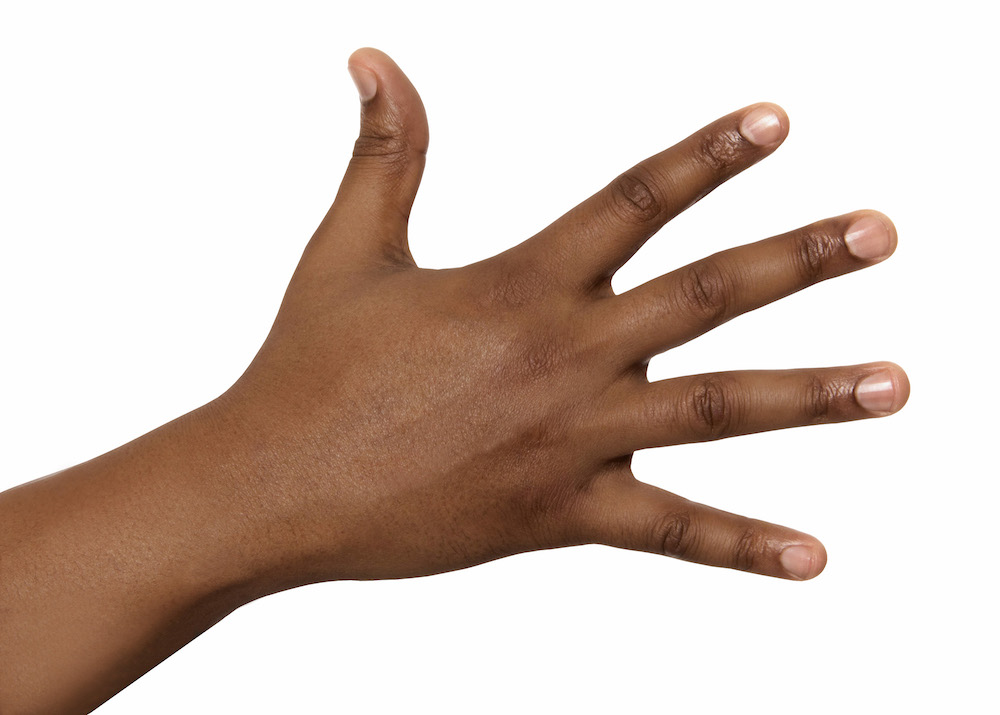
\includegraphics[width=\textwidth,height=\textheight,keepaspectratio]{../inputs/hand_dark.jpg}
  \end{minipage} & 
  \begin{minipage}{.29\textwidth}
    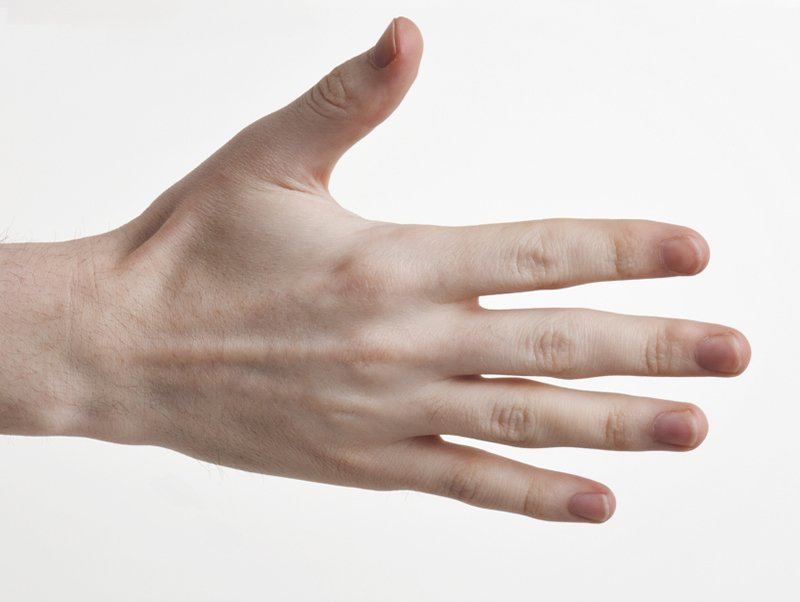
\includegraphics[width=\textwidth,height=\textheight,keepaspectratio]{../inputs/hand_pale.jpg}
  \end{minipage} & 
  \begin{minipage}{.29\textwidth}
    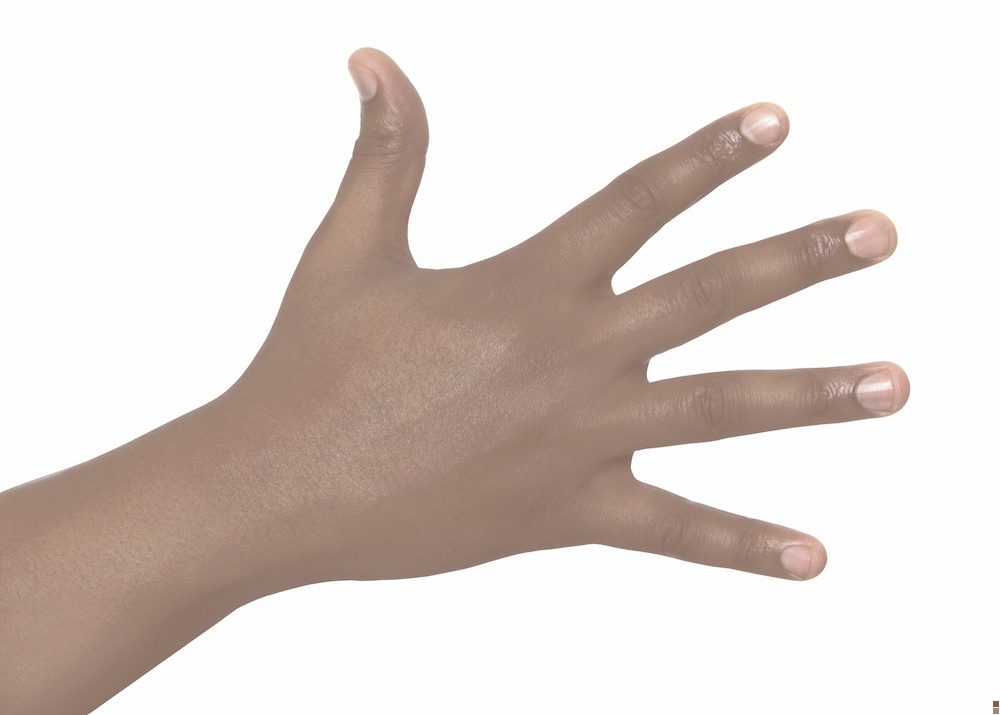
\includegraphics[width=\textwidth,height=\textheight,keepaspectratio]{../rc_test/outputs/debug/hand_dark_to_hand_pale.jpg}
  \end{minipage} \\
\hline
 \end{longtable}

Our results show that images of darker skin tones and smaller changes from the original skin tone to the target colour to begin with (Row \ref{row:boost_test_hand_brown_to_hand_dark}) tend to have better results than images with large changes (Rows \ref{row:boost_test_hand_dark_to_hand_light}, \ref{row:boost_test_hand_brown_to_hand_pale}). In the case of changes towards brighter colours, this is because large changes force bright points in the original image to be truncated at white, and also causes dark regions on the image, such as shadows and grooves, to become significantly brighter and less close to true black, giving the image a ``high-key" appearance (Row \ref{row:boost_test_hand_dark_to_hand_light} and \ref{row:boost_test_hand_brown_to_hand_light}).

In addition, we noted that at this stage the transformation from a dark coloured hand to a very pale hand, or even from a mid-toned hand to a pale hand and vice versa is especially unconvincing. (Row \ref{row:boost_test_hand_brown_to_hand_pale}, also see \ref{row:boost_test_hand_dark_to_hand_pale} and \ref{row:boost_test_hand_pale_to_hand_dark})
